\documentclass[english]{article}
\usepackage[T1]{fontenc}
\usepackage[utf8]{inputenc}
\usepackage{enumerate}
\usepackage{setspace}
\usepackage{amsmath,amssymb,amsthm}
\usepackage{graphicx}
\usepackage{bbm}
\usepackage[round]{natbib}
\usepackage[nohead]{geometry}
\usepackage[bottom]{footmisc}
\usepackage{indentfirst}
\usepackage{endnotes}
\usepackage{graphicx}%
\usepackage{eurosym}
\usepackage{array}
\usepackage{booktabs}
\usepackage{caption}
%\usepackage{subfig}
\usepackage{subcaption}
\usepackage{tabularx}
% \usepackage[hidelinks]{hyperref}
\usepackage{floatrow} %[capposition=top]
\floatsetup{footposition=bottom,capposition=top}
\PassOptionsToPackage{normalem}{ulem}
\usepackage{ulem}
\usepackage{geometry}
\geometry{verbose,tmargin=3cm,bmargin=3cm,lmargin=2.5cm,rmargin=2.5cm}
\bibliographystyle{chicago}


\onehalfspacing


\begin{document}

\title{Rebranding in the French gasoline market: local competitive effects
of price decreases%
\thanks{We thank Philippe Février, Pauline Givord, Daniel Herrera, Laurent
Linnemer, Simon Quantin, two anonymous reporters from the Revue Economique,
as well as seminar participants at CREST, JMA 2015 (Montpellier),
EARIE 2015 (Munich) and JEI 2015 (Alicante) for helpful comments and suggestions.
This article does not reflect views from INSEE or Ecole Polytechnique.%
}}


\author{Etienne Chamayou%
\thanks{CREST and Ecole Polytechnique. 15 Boulevard Gabriel Péri, 92240 Malakoff, France.
Email: etienne.chamayou@ensae.fr%
}, Ronan Le Saout%
\thanks{CREST-INSEE. 18 Boulevard Adolphe Pinard, 75014 Paris France. Email: ronan.le.saout@ensae.fr%
}}

\maketitle
\vspace{-1cm}
\ \\
\ \\
\subsubsection*{Abstract}

Total S.A., the "supermajor" oil company, operates the largest gas station network in France. End of 2011, the company launched a new chain, "Total Access", with the stated goal of recapturing market shares lost to supermarkets. Within two years, 600 gas stations across France were thus rebranded to form the new chain. For half of them, the conversion was accompanied by a sharp c. 10 euro cent per liter drop in prices. The reaction of competitors is studied using difference in differences regressions with daily price data obtained from a comparison website. The measured aggregate response is a slight decrease, of less than one euro cent per liter. It yet conceals increases and decreases in equivalent proportions for the 40\% of the competitors which are found to change their pricing policy by one cent or more. Decreases are mainly implemented by supermarkets, whereas gas stations operated by oil groups and independent networks account for most of the increases. These reactions lead to highlight the role of market segmentation, beyond apparent product homogeneity.

\medskip{}

\date{\noindent \textbf{Codes JEL:} C20, C55, L81.}

\newpage{}


\section{Introduction}

During the 2012 French presidential election campaign, historically high retail gasoline prices stirred a controversy regarding the competitiveness of the market. Following the election, a report was thus requested by the newly formed government (\cite{BEL12}), and claims of insufficient competition in the retail market were found to be without merit. Cited evidence included the development of supermarket networks, the withdrawal of several oil companies, and low estimated net margins, of c. 2 euro cents per liter. The bulk of the then recently observed price increase was attributed to oil price fluctuations, and to the multiplication of costly environmental constraints. The report did however bring little microeconomic evidence regarding competition between gas stations, focusing essentially on profitability. Beyond the price difference of approximately 8 euro cents per liter between supermarket and other gas stations, net margins were estimated to be low for all retailers.%
\footnote{This spread is still to be observed in the gross margin, which measures the difference between before tax price and wholesale cost (including transportation). The net margin, however, once distribution costs are taken into account, is estimated to be similarly low across retailers as the lower gross margin of supermarkets is offset by higher volumes.}.

This paper investigates competition on the French retail gasoline market, using a change in strategy implemented by the largest gas station operator in France, Total S.A. In 2011, the group indeed significantly expanded its "discount" offer through the creation of a new chain, "Total Access". Between September 2011 and December 2014, c. 600 gas stations were consequently rebranded. Among these, 250 used to be operated under the "Elf" brand, originating from a prior merger, and set retail prices which were competitive with those of competing supermarket gas stations. The other gas stations were operated under the "Total" brand and their prices were decreased by 10 euro cents per liter on average, in order to match the "discount" policy of the newly created chain. Using difference-in-difference regressions, we analyse the diesel price reaction of competitors within markets affected by the rebranding.

Following suspicions of asymmetries in upward and downward retail price adjustments to oil price fluctuations, a rich literature on retail gasoline markets has emerged (\cite{ECK13}). Several papers have sought to use merger and acquisition evaluations to shed light on market competitiveness.%
\footnote{\cite{EIN10} and \cite{ANG10}, regarding recent advances in applied industrial economics, express a disagreement as to which methodologies are most appropriate. \cite{EIN10} advocate structural approaches which allow to estimate the demand function and perform merger simulations. \cite{ANG10} criticize the overwhelming use of such approaches as they generally require strong hypotheses. They call for more evidence relying on "simple, transparent empirical methods that trace a shorter route from facts to findings", citing in particular \cite{HAS04}, to which our approach is very similar, as we do not have data on volumes.%
}. Difference in differences analyses have yet yielded contrasted results. \cite{HAS04} and \cite{TAY10} studying the same concentration operation in California, albeit with different data samples, have reached significantly different conclusions: a 5 cent increase per gallon in the former, estimated to be only 1 cent by the latter. \cite{HOU12} has simulated a merger between two retailers in Canada and evaluated its impact ex-post using a difference in differences approach. The paper stresses the importance of heterogeneity across stations and markets, which make results highly sensitive to biases in data sampling. Findings generally suggest weak price adjustment by competitors, conditioned by the structure of competition (presence of independent gas stations in \cite{HAS04}, road traffic and local market power in \cite{HOU12}).
\medskip{}

Data used in this paper allow to overcome the main problems raised by the literature. Price records have a daily frequency which ensure a reasonably fine observation of pricing strategies. Sellers are observed in a virtually exhaustive way, including rebranded stations, other stations operated by Total SA, and competitors. We first estimate aggregate effects using difference in differences regressions while defining markets through radiuses of 1, 3 or 5 km around each rebranded gas station. We then estimate the reaction of each gas station, in order to measure heterogeneity and relax the constraints previously imposed by our market definition. We find that supermarkets have generally implemented small price decreases in reaction to a nearby rebranding, while oil company and independent gas stations have rather slightly increased prices. The heterogeneity of reactions lead to stress the necessity to observe a large sample of gas stations. Focusing on the Paris metropolitan area, we observe that reactions are upwards within Paris and nearby, but downwards as gas stations are located further away (and for France in general). This heterogeneity can be accounted for by the low penetration of supermarket gas stations in Paris. On top of contributing to the understanding of competition in the French retail gasoline market, the paper illustrates how results obtained through difference in difference regressions to evaluate a merger can diverge, depending on market structure and concentration in the observed sample.
\medskip{}

Regarding competition in the French retail gasoline market, results support the idea of a significant market segmentation. On the one hand, a highly price sensitive demand would be catered to by low gross margin gas stations, while other gas stations would serve more loyal or captive customers at high prices. A change in the relative size of those groups would have justified the change in pricing policy implemented by Total. The market would thus be increasingly competitive, yet with a heterogeneous impact on prices, reflecting the persistence of transportation costs and differentiation.
\medskip{}

The first part of the paper describes the French retail gasoline market as well as the rebranding operation implemented by Total SA. The second part provides an overview of the data with descriptive statistics. Finally, the last part details the estimation strategy and the main results.

\section{The French retail gasoline market}

Data cover a three-year time span, from September 2011 to December 2014. Over the period, retail diesel price increases until April 2012 (c. 20 cents to reach c. 1.40 euro per liter after tax), then decreases. Diesel accounts for c. 75\% of household gasoline consumption. Three main types of retailers operate on the market: supermarket chains, oil companies, and independent networks. The price difference between a supermarket gas station and a competitor from another type is generally c. 8 euro cents per liter. Data do not contain information about vertical relations, hence their potential impact is not taken into account in the analysis.

Oil refining has undergone significant restructuring over last years (acquisitions and shutdowns e.g. Petroplus in Normandy in 2012), could have some impact on prices. Taxes account for c. 60$\%$ of retail prices. They consist of a fixed components (exhibiting slight variations across regions) and the VAT.
\medskip{}

The \cite{BEL12} report relies on the evolution of the gas station network as well as estimations of profitability (net margin of 0.2 to 2 euro cents per liter) to support the thesis of a highly competitive market. The total number of gas stations
has indeed plummeted from 40,000 to 12,000 between 1980 and 2012. Meanwhile, the market share of oil companies has kept decreasing, while supermarkets were expanding their networks. Gas stations operated by supermarkets account for c. 50\% of the total number of gas stations over the studied period, while their market share is c. 60\%.
\medskip{}

Upon creating "Total Access", Total S.A. has stated that its goal was to recapture market shares lost to supermarkets. The idea was to associate the development of "discount" offer with the quality brand image. Before the creation, Total SA distributed gasoline through three chains: Total, Elf and Elan. The Elan chain is essentially to be found where both demand and competition are low, typically in rural areas. It was not impacted by the rebranding operation. The Elf chain was inherited from a prior merger, and was until then the "discount" chain of Total SA. Stations were rebranded "Total Access" and the pricing policy was left unchanged. Some minor modifications may have affected stations such as the addition of a premium gasoline. Finally, as regards former Total gas stations, the rebranding was accompanied by a significant decrease in prices, and occasionally some upgrades such as the the addition of some pumps. Gas station amenities may have been marginally reduced, for instance through a shrinkage in the number of products available at the gas station shop.
\medskip{}

While Total S.A. has largely advertised the creation of its new chain, the identity of affected gas stations was not disclosed until their respective rebranding. The pace of the development of the network has been fairly regular following the announcement. Required renovation works last one to two weeks and were reported to cost between one and two million euros for each gas station. Total S.A. has also mentioned that the magnitude of the price decreases was decided based on each gas station market environment. At the end of the studied period, Total Access gas stations could be found across all regions of France.%
\footnote{Philippe Callejon, in charge of the creation of the chain, has given several interviews to explain the choice to convert classic Total stations to Total Access. ``A test was implemented over 18 months within 45 cities. This test period was crucial. Prices, through a 9 cent decrease, were aligned on market prices. We have then examined at the impact of the price decrease on the economic model of gas stations. Conclusion: in order to make up for the price decrease, we must increase volumes. Very piratically, we need gas stations big enough to have several pumps. They must be located on highly frequently roads so that there are enough potential customers. As a matter of fact, within the Total network, some gas stations are located on roads were the traffic is low. We have no influence on such elements, as well as the fact that it is nearly impossible to obtain the authorization to open a new gas station. The test has thus confirmed the necessity to create a network with two offers: gas stations with competitive prices, in periphery, where higher volumes resulting from potential demand can make up for the decrease in price, and proximity gas stations, with classic prices.''%
}.

\section{Data and descriptive statistics}

Data come from the price comparison website www.prix-carburants.gouv.fr, on which French gas stations are legally required to keep prices up to date since 2007. The accuracy of data is ensured by regular  controls which can lead to financial penalties. Small gas stations are no subject to the legal obligation. As a consequence, 10,200 gas stations out of 12,000 over France are observed. Other price comparison website exists but tend to be less exhaustive as the legal obligation imposed on retailers only concerns the governmental price comparison website. \medskip{}

The analysis is based on daily price records spanning slightly more than three years, from September 4, 2011 to December 4, 2014. Some short periods are missing due to technical issues encountered during data collection (cf. Figure~\ref{fig:diesel_and_brent}). Gas stations located on the island of Corsica were excluded (130 gas stations) as well as gas stations located on highway (less than 500) since they are part of specific markets. Some gas station for which observations were too short or price dynamics looked suspicious, mainly because of excessive rigidity, were also discarded. We also drop gas stations which already compete with a Total Access gas station as of September 2011 (i.e. when the rebranding occurred prior to the beginning of our study) or which compete with a gas station for which the observed price change is below 4 euro cents per liter (500 gas stations). Former Total stations for which the price change is small are likely gas stations which were used during the test phase, meaning that the price decrease has occurred before the rebranding (cf. comments on Figure~\ref{fig:price_dist_total_ba}). In order to estimate a potential effect of the rebranding on other gas stations operated by Total SA, we include them in the analysis. About 300 are located within a distance of 5 km of a Total-Total Access, and 100 within 5 km of an Elf-Total Access. Finally, we only keep gas stations which are located within 10 km from a rebranded gas station (cf. part 4 on the estimation strategy). About 4,700 gas stations are dropped based on this filter, leaving us with c. 3,100 gas stations and c. 3 million price observations. About 1,300 are considered to compete with a Total-Total Access gas station and 400 with an Elf-Total Access. Other gas stations located within 5 to 10 km from a Total Access are used as a control group in our difference in differences analysis, as they are assumed to not directly compete with Total Access gas stations. Out data include gas station characteristics and locations. Census data and other publicly available data were added based on the municipality of each gas station. For each of them, we built several variables describing competition such as the distance to the closed competitor and the number of competitors located within a 1, 3 or 5 km distance.
\medskip{}

\begin{figure}[H]
    \caption{Evolution of diesel and Brent prices}
		\label{fig:diesel_and_brent}
%\begin{center}
\includegraphics[scale=0.4]{graphs/macro_trends.png}
%\end{center}
\flushleft
{\small{}\uline{Reading Note}}{\small{}:
Diesel prices are average retail prices excluding taxes. Some periods are missing as prices could not be collected for technical reasons.}{\small \par}
{\small{}\uline{Source}}{\small{}: Governmental website for diesel prices; UFIP website for Brent.}\medskip{}
\end{figure}

Gas station chain changes are observed in the data, and were validated with publications of Total SA. A renovation work period is associated with a rebranding and lasts about 15 days, during which the gas station remains closed. The measure of the price effect via a difference in differences for Total-Total Access and Elf-Total Access gas stations as well as for other Total SA gas stations correspond to the direct effect, i.e. a decision by Total SA.%
\footnote{Only difference in difference results obtained with a national control are presented. Robustness checks were performed with regional controls and at a series level (cf part 4.1) and provided similar results.%
}. The direct effect analysis is meant to verify that price decreases were actually implemented together with the rebranding, and whether Total SA may have changed its pricing policy for other gas stations at the same time without communicating about it.
\newpage{}

\begin{figure}[H]
    \caption{Detection of a change in pricing policy for a Total Access gas station}
		\label{fig:margin_change_detection}
%\begin{center}
\includegraphics[scale=0.4]{graphs/margin_change_detection.png}
%\end{center}
\flushleft
{\small{}\uline{Reading Note}}{\small{}: } The grey line represents the prices $\mathrm{P}_{t}$ of a Total Access gas station. The black line represents the national average price $\overline{\mathrm{P}}_{t}$. The detected date for the change is represented by the vertical line.\medskip{}
\end{figure}

The price series of a rebranded Total gas station is shown on Figure~\ref{fig:margin_change_detection}. Prices are initially above the national average. From December 2013 on,
following a c. 8 euro cent decrease in the pricing policy, prices are consistently below the national average. The temporal discontinuity is easily seen graphically and can been detected statistically as well. In the data, we observe 325 chain changes from Total to Total Access accompanied by a price decrease of 4 cents or more (i.e. 2 euros for a 50L tank), 250 chain changes from Elf to Total Access, and 350 other changes (within 5 km of a Total Access gas station). Approximately 200  are associated with a change from Esso to Esso express, for which a small price decreasee is observed (below 2 cents). For other gas
stations (except for very few of them), we do not observe any adjustment in prices. Changes essentially result from harmonization within supermarket chains. We excluded these gas stations from the analysis and checked that results were not affected. The conversions of Total and Elf gas stations occur progressively over the studied period. Figure 3 displays the distributions of Total SA gas station prices at the beginning and at the end of the period. In the latter, the distribution can be seen to be bimodal, reflecting the existence of the "discount" networks besides other gas stations with "classic" Total prices. The graph also displays gas stations which already set low prices in September 2011 before their conversion, and were likely part of the test phase. These gas stations were identified through difference in differences regressions and excluded from the analysis. Results of the difference in differences analysis for rebranded Total
and Elf gas stations, as well as for nearby Total SA gas stations, are reported in Table 1. Rebranded Total gas station are found to drop prices by an average 10 cents. No substantial decrease is observed for former Elf gas stations and for nearby Total SA gas
stations. Table 6 (cf. infra) details the distribution of price policy changes measured through an individual level analysis. The median price decrease for former Total stations is 10 cents, the ninth decile is 7 cents and the first decile 12 cents. Regarding former Elf gas stations, only one observation displays a price policy change above 2 cents (3 cent increase).

\subsubsection*{Table 1: Total Access rebranding aggregate direct effets (euro cents) - DD regressions}

\begin{center}
\begin{footnotesize} %
\begin{tabular}{l|ccc}
\multicolumn{1}{l}{} &  &  & \tabularnewline
\hline
\hline
 & \textbf{(1)}  & \textbf{(2)}  & \textbf{(3)}\tabularnewline
 & \textbf{Price}  & \textbf{Price}  & \textbf{Price}\tabularnewline
 & \textbf{5 km}  & \textbf{3 km}  & \textbf{1 km}\tabularnewline
\hline
\textbf{Total-Total Access}  & -9.89{*}{*}{*}  & -9.88{*}{*}{*}  & -9.87{*}{*}{*}\tabularnewline
 & (0.17)  & (0.17)  & (0.16) \tabularnewline
\textbf{Total SA gas stations}  & -0.17  & -0.19{*}  & -0.09\tabularnewline
\textbf{close to Total-Total Access}  & (0.10)  & (0.10)  & (0.25)\tabularnewline
\hline
\textbf{Elf-Total Access}  & -0.08{*}  & -0.08  & -0.07\tabularnewline
 & (0.05)  & (0.05)  & (0.05)\tabularnewline
\textbf{Total SA gas stations}  & 0.08  & -0.01  & -0.14\tabularnewline
\textbf{close to Elf-Total Access}  & (0.12)  & (0.13)  & (0.13)\tabularnewline
\hline
\textbf{Intercept}  & 136.10{*}{*}{*}  & 135.81{*}{*}{*}  & 135.15{*}{*}{*}\tabularnewline
 & (0.17)  & (0.17)  & (0.17)\tabularnewline
\hline
\textbf{Nb. Obs.}  & 301.500  & 282.231  & 249.040\tabularnewline
\textbf{Adj. R2}  & 0.967  & 0.967  & 0.967\tabularnewline
\hline
\hline
\multicolumn{1}{l}{} &  &  & \tabularnewline
\end{tabular}\end{footnotesize}
\par\end{center}

{\small{}\uline{Reading note}}{\small{}: } Prices include VAT. Columns 1, 2 and 3 correspond to the following regression: $\mathrm{P}_{it}=\mathrm{\gamma}\cdot Treatment_{it}+\mathrm{\mu}_{i}+\mathrm{\eta}_{t,c}+\mathrm{\varepsilon}_{it}$ with $\mathrm{\eta}_{t,c}$ the temporal effects of a control group $c$, $\mathrm{\mu}_{i}$ gas station fixed effects, $\mathrm{\gamma}$ the effect of the rebranding ($Treatment_{it}$ is a dummy which takes value 1 after the rebranding). The control group includes gas stations within a 5 to 10 km distance from Total Access gas stations. Errors are clustered at the regional level. Significance thresholds: {*}{*}{*} 1\%, {*}{*} 5\%, {*} 10\%.\medskip{}

\begin{figure}[H]
\centering
\caption{Distributions of Total prices before and after rebranding}
\label{fig:price_dist_total_ba}
\begin{subfigure}[t]{.49\columnwidth}
\centering
\includegraphics[scale=0.43]{graphs/price_dist_total_before.png}
\caption[short]{September 4, 2011}
\end{subfigure}
\begin{subfigure}[t]{.49\columnwidth}
\centering
\includegraphics[scale=0.43]{graphs/price_dist_total_after.png}
\caption[short]{December 4, 2014}
\end{subfigure}
\flushleft
{\small{}\uline{Reading Note}}{\small{}: In black, Total gas stations which are rebranded Total Access. In grey, Total gas stations which are not rebranded.}{\small \par}
\end{figure}

\medskip{}

The main goal of this paper is to study the price reaction of competitors to the creation of Total Access. Such an analysis requires a definition of competition, which is a well know crucial issue in such a difference in differences analysis. Indeed, the compositions of the treatment and control groups depend on this definition. The usual procedure implemented in the literature consists in relying on a distance, which can also be defined in several ways, and to check the robustness of results to perturbations in the definition. \cite{HAS04} uses a radius of one mile (1.8 km), based on interviews with retailers, to study the impact on prices of a merger between two chains in California. The robustness of results is checked with alternative radiuses of 0.5 and 1.5 miles. The control group is composed by non affected gas stations located within the urban area (San Diego or Los Angeles). \cite{BRU15} measure the price effect of the installation of automated gas stations in the Netherlands. The intensity of competition is captured by the number of gas stations within 2 and alternatively 5 km. In order to study a merger between two chains in Canada, \cite{HOU12} uses a structural approach based on a Hotelling model. The definition of markets essentially relies on commuting patterns. Results of the structural approach are compared with results obtained via a difference in differences analysis which use a distance based on time (30 seconds, 1 or 1.5 minute). Results are overall consistent but sensitive to the market structure and the analyzed sample.

We therefore consider a 5 km radius to be a relatively broad approach to competition and perform robustness checks with 1 and 3 km radiuses. We also perform a specific analysis for the Paris metropolitan area, where we can distinguish the city of Paris, its close surroundings, and the whole region.

Market price variations over time are captured by daily fixed effects. Their estimates are almost perfectly correlated with wholesale diesel cost. We perform our analysis with prices including VAT in order to obtain the effect for consumers. Regressions with pre-tax prices yield similar results (closer to the gross margin of retailers), c. 20\% smaller in value due to the VAT.
\medskip{}

Table 2 describes the competitive environment of a Total-Total Access gas stations. Gas stations which are rebranded are generally located in markets which exhibit above average competitive pressure. Their closest competitors is 1.2 km away while it is 1.8 km away for others. Their number of competitors is higher regardless of the size of the considered radius (1, 3 or 5 km). In "Ile-de-France", the administrative region which contains Paris, the city and its close surroundings contrast sharply with the broader surroundings. On the one hand, the number of competitors within 5 km is more than twice higher and the distance to the closest competitor is about twice smaller in the former than in the latter. On the other hand, the distance to a supermarket gas station is greater, with respective 2.2 km and 1.6 km average distance. The market structure is therefore different in and close to Paris as it is characterized by a higher gas station density but less supermarket gas stations. The broader surroundings of Paris are rather similar to France as a whole in terms of market structure. The relevant definition of markets is therefore likely to depend on location, typically smaller for Paris. As a consequence, we develop an estimation strategy which provides flexibility regarding the definition of competition.
\medskip{}

\subsubsection*{Table 2: Competitiveness of Total gas station markets}

\begin{center}
\begin{scriptsize} %
\begin{tabular}{lccccccc}
 &  &  &  &  &  &  & \tabularnewline
\hline
\hline
{\tiny{}{} } &  & \textbf{\tiny{}Distance}{\tiny{} } & \textbf{\tiny{}Distance}{\tiny{} } & \textbf{\tiny{}Distance}{\tiny{} } & \textbf{\tiny{}Nb}{\tiny{} } & \textbf{\tiny{}Nb}{\tiny{} } & \textbf{\tiny{}Nb }\tabularnewline
{\tiny{}{} } &  & \textbf{\tiny{}closest}{\tiny{} } & \textbf{\tiny{}closest}{\tiny{} } & \textbf{\tiny{}closest}{\tiny{} } & \textbf{\tiny{}competitor}{\tiny{} } & \textbf{\tiny{}competitor}{\tiny{} } & \textbf{\tiny{}competitors}\tabularnewline
{\tiny{}{} } & \textbf{\tiny{}Nb. Obs.}{\tiny{} } & \textbf{\tiny{}competitors}{\tiny{} } & \textbf{\tiny{}supermarkets}{\tiny{} } & \textbf{\tiny{}Total}{\tiny{} } & \textbf{\tiny{}1 km}{\tiny{} } & \textbf{\tiny{}3 km}{\tiny{} } & \textbf{\tiny{}5 km }\tabularnewline
\hline
\textbf{\tiny{}TOTAL}{\tiny{} } & {\tiny{}1787 } & {\tiny{}1.64 } & {\tiny{}2.05 } & {\tiny{}5.55 } & {\tiny{}0.71 } & {\tiny{}3.39 } & {\tiny{}6.96 }\tabularnewline
\textbf{\tiny{}- not Total Access}{\tiny{} } & {\tiny{}1413 } & {\tiny{}1.75 } & {\tiny{}2.18 } & {\tiny{}6.01 } & {\tiny{}0.69 } & {\tiny{}3.17 } & {\tiny{}6.50 }\tabularnewline
\textbf{\tiny{}- Total Access}{\tiny{} } & {\tiny{}374 } & {\tiny{}1.21 } & {\tiny{}1.55 } & {\tiny{}3.85 } & {\tiny{}0.81 } & {\tiny{}4.23 } & {\tiny{}8.70 }\tabularnewline
\hline
\textbf{\tiny{}ELF}{\tiny{} } & {\tiny{}269 } & {\tiny{}1.17 } & {\tiny{}1.60 } & {\tiny{}2.57 } & {\tiny{}0.86 } & {\tiny{}4.68 } & {\tiny{}10.28 }\tabularnewline
\hline
\textbf{\tiny{}Paris and closest surroundings}{\tiny{} } & {\tiny{}137 } & {\tiny{}0.83 } & {\tiny{}2.22 } & {\tiny{}1.07 } & {\tiny{}1.11 } & {\tiny{}9.36 } & {\tiny{}24.76}\tabularnewline
\textbf{\tiny{}Paris broader surroundings}{\tiny{} } & {\tiny{}180 } & {\tiny{}1.64 } & {\tiny{}2.08 } & {\tiny{}3.00 } & {\tiny{}0.52 } & {\tiny{}3.51 } & {\tiny{}8.54}\tabularnewline
\hline
\hline
 &  &  &  &  &  &  & \tabularnewline
\end{tabular}\end{scriptsize}
\par\end{center}

{\small{}\uline{Reading Note}}{\small{}: }On average, the 1787 Total gas stations (whether rebranded or not) are located 1.64 km away from their closest competitor. Their average number of competitors whithin 3 km is 3.39. The 137 Elf and Total gas stations (whether rebranded or not) located in Paris and its closest surroundings are on average 2.22 km away from a supermarket.
\medskip{}

Table 3 describes price level determinants in level on a given day%
\footnote{Retail prices are primarily determined by crude oil prices. Studying prices on a given day allows to shed lights on the influence of observable variables describing gas stations and their markets.%
}. Supermarket gas stations are on average 5 to 7 cent cheaper than other gas stations and this single distinction accounts for c. 56\% of the price variance on a given day. The presence of a shop, car services (e.g. car wash) or the availability of premium gasoline generally imply a 0.5 to 1.5 cent higher price. On the other hand, the presence of
automated pumps is associated with a 0.7 cent lower price. Prices are generally higher when the population density is lower but also in Paris and its close surroundings. Competition is found to have a significant impact (distance to the closest supermarket, number of competitors within 3 km), yet of low magnitude and therefore likely not noticeable for consumers. Prices are also slightly higher when concentration is higher. Results are consistent with \cite{HOS08},
which find gas station prices in Washington DC to be largely accounted for by gas station chains, characteristics, market demand structure, and to a lesser extent by competition. \cite{ZIM12} has studied the impact on prices of the development of supermarket gas stations in the US. However, the situation is yet different as these account for less than 10\% of gas stations in the US. Tables 3 accounts for the impact of observed gas station characteristics on the decision by Total S.A. to rebrand its Total gas stations Total Access or not. Findings allow to confirm part of the communication of Total S.A. Changes are more frequent in large urban areas (except for Paris), when the number of competitors is high and the distance to a supermarket is low. Changes are less likely inside Paris and in rural areas. On average, a gas station located in Paris or its close surroundings is 10\% less likely to be rebranded.

The possibility to pay at the pump, generally associated with above average volumes, implies a 17\% increase in the probability of rebranding. Converted Elf gas stations are also generally located in urband areas, in particular around Paris, and are often equipped with pay at the pump systems. Their number of competitors is relatively normal compared to the overall Total gas station population. They however differ significantly as regards the presence of premium gasoline (26\% less likely in an Elf gas station). The switch from Elf to Total Access could therefore have meant an increase in perceived quality, if premium gasoline has been made available. All these characteristics do not allow to predict which stations were going to be rebranded (the sensitivity i.e. the percentage of changes correctly predicted is c. 10\%). This supports the hypothesis that competitors could not anticipate which gas stations were likely to be rebranded Total Access. \medskip{}

\subsubsection*{Table 3: Key determinants of prices and Total-Total Access conversions, and Elf gas station specificities}

\begin{center}
\begin{footnotesize} %
\begin{tabular}{l|cccccc}
\multicolumn{1}{l}{} &  &  &  &  &  & \tabularnewline
\hline
\hline
 & \textbf{(1)}  & \textbf{(2)}  & \textbf{(3)}  & \textbf{(4)}  & \textbf{(5)}  & \textbf{(6)}\tabularnewline
 & \textbf{Price}  & \textbf{Price}  & \textbf{Price}  & \textbf{Price}  & \textbf{Total Access}  & \textbf{Elf}\tabularnewline
 & \textbf{OLS}  & \textbf{OLS}  & \textbf{OLS}  & \textbf{OLS}  & \textbf{Probit}  & \textbf{Probit}\tabularnewline
\hline
\textbf{Supemarkets}  & -7.15{*}{*}{*}  & -7.10{*}{*}{*}  & -7.09{*}{*}{*}  & -5.66{*}{*}{*}  &  & \tabularnewline
\textbf{\textit{(Ref. Oil companies)}}  & (0.31)  & (0.33)  & (0.33)  & (0.42)  &  & \tabularnewline
\hline
\textbf{Dist. to closest}  &  & 0.07{*}{*}  & 0.05{*}{*}  & 0.07{*}{*}{*}  & -0.011{*}  & -0.009{*}{*}{*}\tabularnewline
\textbf{supermarket (km)}  &  & (0.03)  & (0.02)  & (0.02)  & (0.006)  & (0.003)\tabularnewline
\textbf{Nb competitors}  &  & -0.14{*}{*}{*}  & -0.11{*}{*}{*}  & -0.10{*}{*}{*}  & 0.015{*}{*}{*}  & -0.000\tabularnewline
\textbf{within 3 kms}  &  & (0.05)  & (0.03)  & (0.04)  & (0.005)  & (0.003)\tabularnewline
\textbf{Nb same group gas stations}  &  & 0.35{*}{*}{*}  & 0.32{*}{*}{*}  & 0.25{*}{*}{*}  & -0.011  & 0.007{*}{*}{*}\tabularnewline
\textbf{with 3 kms}  &  & (0.08)  & (0.06)  & (0.05)  & (0.009)  & (0.003)\tabularnewline
\hline
\textbf{Rural area}  &  &  & 0.49{*}{*}{*}  & 0.53{*}{*}{*}  & -0.074{*}{*}  & -0.049{*}{*}\tabularnewline
\textbf{\textit{(Ref. Other urban area)}}  &  &  & (0.08)  & (0.09)  & (0.032)  & (0.022)\tabularnewline
\textbf{Urban area of more than}  &  &  & -0.47{*}{*}{*}  & -0.47{*}{*}{*}  & 0.084{*}{*}{*}  & 0.025{*}\tabularnewline
\textbf{100,000 inhabitants (except for Paris)}  &  &  & (0.13)  & (0.13)  & (0.032)  & (0.015)\tabularnewline
\textbf{Paris and surroundings}  &  &  & 1.11{*}{*}  & 1.13{*}{*}  & -0.106{*}{*}  & -0.056{*}{*}{*}\tabularnewline
 &  &  & (0.40)  & (0.41)  & (0.040)  & (0.014)\tabularnewline
\hline
\textbf{Pay at the pump}  &  &  &  & -0.73{*}{*}{*}  & 0.171{*}{*}{*}  & 0.158{*}{*}{*}\tabularnewline
 &  &  &  & (0.12)  & (0.020)  & (0.011)\tabularnewline
\textbf{Premium gasoline}  &  &  &  & 1.46{*}{*}{*}  & -0.070  & -0.258{*}{*}{*}\tabularnewline
 &  &  &  & (0.13)  & (0.065)  & (0.053)\tabularnewline
\textbf{Shop}  &  &  &  & 0.46{*}{*}{*}  & 0.114{*}  & 0.030\tabularnewline
 &  &  &  & (0.14)  & (0.047)  & (0.045)\tabularnewline
\textbf{Car repair}  &  &  &  & 0.54{*}{*}{*}  & 0.015  & -0.075{*}\tabularnewline
 &  &  &  & (0.15)  & (0.072)  & (0.047)\tabularnewline
\hline
\textbf{Intercept}  & 139.60{*}{*}{*}  & 139.66{*}{*}{*}  & 139.68{*}{*}{*}  & 138.12{*}{*}{*}  &  & \tabularnewline
 & (0.18)  & (0.35)  & (0.30)  & (0.51)  &  & \tabularnewline
\hline
\textbf{Nb. Obs.}  & 7417  & 7417  & 7417  & 7417  & 1582  & 1770\tabularnewline
\textbf{Adj. R2}  & 0.560  & 0.575  & 0.582  & 0.607  & 0.131  & 0.222\tabularnewline
\textbf{Reference probability}  &  &  &  &  & 0.219  & 0.112\tabularnewline
\textbf{Sensitivity}  &  &  &  &  & 0.094  & 0.139\tabularnewline
\hline
\hline
\multicolumn{1}{l}{} &  &  &  &  &  & \tabularnewline
\end{tabular}\end{footnotesize}
\par\end{center}

{\small{}\uline{Reading Note}}{\small{}: } Columns 1 to 4 account for the regressions of gasoline prices (cents, including taxes) on September 9, 2011. Column 5 describes the determinants of a Total-Total Access rebranding (marginal effects of a probit model run with all Total gas stations). Column 6 accounts for the specificities of the Elf brand (marginal effects of a probit model run with all Total and Elf gas stations). Regional controls are included. Errors are clustered at the regional level. Significance threshold: {*}{*}{*} 1\%, {*}{*} 5\%, {*} 10\%.

\section{Estimation and results}

\subsection{Estimation strategy}

We perform a difference in differences analysis, close to the approach of \cite{HAS04}. We compare the evolutions in prices, before and after the rebranding, between competitors of rebranded gas station and control gas stations.\medskip{}

Prices are sticky (\cite{GAU15}), typically remaining unchanged during 5 to 7 days. We perform our difference in differences regressions with weekly data (Friday prices) as a conservative approach
limiting the overconfidence typically induced by stickiness. Competition is successively defined by circles of radius 1, 3 and 5 km.%
\footnote{We obtain similar results when we consider all gas stations within 10 km to be competitors, and include all others in the control group. Performing the analysis with daily data (or another day of week)
also does not substantially affect results. It essentially increases the significance of estimated coefficients.%
}. We first estimate an aggregate model with treatment dummies $Treatment_{it}$ for Total-Total Access and Elf-Total Access changes, that we also cross with retailer type (oil company and independent vs. supermarkets). Regarding gas stations which are found to compete with several Total-Total Access gas stations, we take into account the date of the first conversion.%
\footnote{Taking into account the date of change of the closest gas station does not affect results.%
}. When a gas station is found to compete both Total-Total Access and Elf-Total Access gas stations, we do not take into account the Elf-Total Access rebranding. The expected impact of an Elf-Total Access conversion is indeed limited, given the absence of change in the pricing strategy. The model writes as follows, for a gas station $i$ and a date $t$:

\begin{equation}
\mathrm{P}_{it}=\mathrm{\gamma}\cdot Treatment_{it}+\mathrm{\mu}_{i}+\mathrm{\eta}_{t,c}+\mathrm{\varepsilon}_{it}\label{eq:1}
\end{equation}

\medskip{}

The fixed effect $\mathrm{\mu}_{i}$ controls for unobserved gas station characteristics which lead to persistent differences in prices. Including such fixed effects is necessary to avoid biases that could arise if treated gas stations are more likely to be of a certain type (e.g. oil or independent) associated with a specific pricing strategy. Time fixed effects $\mathrm{\eta}_{t,c}$ are included for each date $t$ and control group $c$. They control for shocks common to all gas stations, whether they are treated or belong to the control group. Finally, $\mathrm{\varepsilon}_{it}$ accounts for unobserved idiosyncratic shocks.
\medskip{}

The validity of the estimation strategy relies on the existence of a trend common to the treatment and control groups. In the absence of treatment, price trends would have then been similar. This means that
$\mathbb{E}\left(Treatment_{it}\cdot\mathrm{\varepsilon}_{it}\left|\mathrm{\mu}_{i},\mathrm{\eta}_{t,c}\right.\right)=0$. French gasoline price variations essentially depend on oil price fluctuations, across all local markets. The hypothesis that price dynamics should be similar for nearby gas stations (within 5 to 10 km of a Total Access gas station) thus seems reasonable. Nevertheless, given the relatively large size considered for the market, it could turn out not to be verified. For instance, it can be locally wrong if a refinery or a gasoline depot has been closed. We thus build control groups within each region. Finally, since gas stations are converted progressively over the whole period, we can implement an internal control i.e. define the control group at any point in time as the gas stations which have not been treated yet. Since all these methods give similar results, we only include outputs obtained with one control group at the national level.
\medskip{}

A major shortcoming of the aggregate approach is the fact we obtain an average effect, which is therefore sensitive to the definition of markets and the studied sample. With two well identified retailer types, and therefore various local market structures, it is meanwhile reasonable to expect heterogeneity among affected gas stations. We therefore estimate individual treatment effects with the following specification:

\begin{equation}
\mathrm{P}_{it}=\mathrm{\gamma}_{i}\cdot Treatment_{it}+\mathrm{\mu}_{i}+\mathrm{\eta}_{t,c}+\mathrm{\varepsilon}_{it}\label{eq:2}
\end{equation}

\medskip{}

The coefficient of interest $\mathrm{\gamma}_{i}$ is therefore estimated for each gas station, thanks to the richness of the date and the close relationship generally observed between gas station prices and their main determinant, the Rotterdam wholesale gasoline price. The individual approach allows to investigate heterogeneity in reactions and to discuss the robustness of results to our definition of market. In terms of methodology, it is close to a temporal discontinuity regression (\cite{AUF11}), for which the randomization hypothesis boils down to the necessity for the conversion not to have been expected by competitors. This hypothesis seems reasonable since Total has not announced specifically which gas stations were going to be rebranded.\medskip{}

In order to deal with temporal and geographical correlation of difference in differences estimators, we allow the error terms to be correlated within each region and on each date  (\cite{BER04}), or simply within each region (\cite{CAM15}). We have also performed the analysis by running one regression for each gas station with the Newey-West estimator in order to allow for temporal autocorrelation. Results displayed come from the aggregate estimation, with correlation allowed within regions. They are robust to the previously mentioned variations in specification. Generally, all measured increases or decreases whose value is above 1 cent are found to be statistically significant.

\subsection{Results}

The retail gasoline market has been the topic of a rich literature, motivated at first by questions regarding the reactions of retail prices to variations in crude oil prices. Gas stations were indeed suspected to perform downwards adjustments at a slower pace than upwards adjustments. Access to increasingly large and precise data has allowed to test the various models of oligopolistic competition, legitimated by a strong heterogeneity in observed price patterns. \cite{ECK13} has documented the existence of “Edgeworth” cycles, not caused by wholesale cost fluctuations but related to the market structure. \cite{CHA11} have provided evidence of significant price dispersion, reflecting a lack of information about prices by consumers. Finally, evaluating the impact of a merger, \cite{HOU12} has shown the impact of commuter flows, and thus transportation costs, on competition.\medskip{}

The French market differs in a significant way from previously cited market due to the strong penetration of supermarkets. It is indeed composed, in virtually equal shares, of low price gas stations, often operated by a supermarkets and with few amenities, and high price gas stations offering more amenities and enjoying more brand awareness (except for few completely independent gas stations). The studied Total-Total Access conversions are accompanied by an 8 to 10 euro cent per liter decrease in price, which essentially corresponds to the difference in price observed between low and high price gas stations. At the time of the creation of Total Access, the Total group has stated that it had selected gas stations for which higher volumes resulting from price decreases were expected to make up for the loss of margin. Given the proximity of supermarket competitors, this leads to think that such gas stations were likely selling to loyal or captive customers, and are supposed, upon rebranding, to benefit from a larger demand, including more price sensitive customers.\medskip{}

There are no significant elements which support the idea that Total Access has effectively reduced its operating costs within rebranded gas stations. It seems therefore reasonable to rather expect a change in demand to account for Total’s strategical choice. Consumers can indeed be expected to have become increasingly price sensitive. The three main differentiation dimensions of the market can be reminded to be location, brand and amenities (presence of a shop, car wash facility etc.).\medskip{}

Taking into account the characteristics and dynamics of the French market leads to forge several hypotheses regarding the reactions of competitors of converted gas stations. In a Hotelling model, supermarket gas stations, confronted to fiercer competition (reduced differentiation) can be expected to decrease prices. The relatively low estimated margins however do not allow for large price cuts. The case of oil company and independent gas stations is more ambiguous, depending on consumer preferences and the local market structure. On the one hand, increased competition may drive prices downwards. On the other hand, capacity constraints implied by the number of pumps, or an unfavorable location, may hamper the ability of a gas station to be profitable at prices set by supermarkets (resp. Total Access) gas stations. An affected gas station may thus be left with a demand composed virtually exclusively by captive or loyal customers, whereas it previously attracted some mildly price sensitive customers. In such a situation, an increase in prices could result from a nearby conversion. Regarding conversions from Elf to Total Access, even in the absence of change in the pricing policy, the creation of a new chain could imply an increase in perceived quality, in particular when premium gasoline is now available on top of basic gasoline. A decrease in prices could therefore be observed among competitors. However, the previous mentioned mechanism leading to an increase could also apply, in particular in areas where both Elf and Total operated. \medskip{}

\newpage{}

\subsubsection*{Table 4: Aggregate reactions of competitors to Total Access rebranding (cents) - Difference in differences regressions}

\begin{center}
\begin{footnotesize} %
\begin{tabular}{l|cccccc}
\multicolumn{1}{l}{} &  &  &  &  &  & \tabularnewline
\hline
\hline
 & \textbf{(1)}  & \textbf{(2)}  & \textbf{(3)}  & \textbf{(4)}  & \textbf{(5)}  & \textbf{(6)}\tabularnewline
 & \textbf{Price}  & \textbf{Price}  & \textbf{Price}  & \textbf{Price}  & \textbf{Price}  & \textbf{Price}\tabularnewline
 & \textbf{5 km}  & \textbf{5 km}  & \textbf{3 km}  & \textbf{3 km}  & \textbf{1 km}  & \textbf{1 km}\tabularnewline
\hline
\textbf{Total-Total Access competitors}  & -0.23{*}{*}  & -0.55{*}{*}{*}  & -0.31{*}{*}{*}  & -0.59{*}{*}{*}  & -0.41{*}{*}{*}  & -0.53{*}{*}{*}\tabularnewline
 & (0.08)  & (0.13)  & (0.07)  & (0.07)  & (0.14)  & (0.08)\tabularnewline
\textbf{Oil company}  &  & 0.40  &  & 0.80{*}{*}{*}  &  & 0.87{*}{*}{*}\tabularnewline
\textbf{\textit{(Ref. Supermarkets)}}  &  & (0.26)  &  & (0.15)  &  & (0.13)\tabularnewline
\hline
\textbf{Elf-Total Access competitors}  & 0.17  & -0.19  & 0.16  & -0.18{*}{*}{*}  & -0.08  & -0.15{*}{*}\tabularnewline
 & (0.10)  & (0.15)  & (0.12)  & (0.06)  & (0.18)  & (0.06)\tabularnewline
\textbf{Oil company}  &  & 0.25  &  & 0.85{*}{*}{*}  &  & 0.85{*}{*}{*}\tabularnewline
\textbf{\textit{(Ref. Supermarkets)}}  &  & (0.34)  &  & (0.19)  &  & (0.15)\tabularnewline
\hline
\textbf{Intercept}  & 133.19{*}{*}{*}  & 133.20{*}{*}{*}  & 133.34{*}{*}{*}  & 133.34{*}{*}{*}  & 133.72{*}{*}{*}  & 133.72{*}{*}{*}\tabularnewline
 & (0.20)  & (0.19)  & (0.19)  & (0.18)  & (0.17)  & (0.17)\tabularnewline
\hline
\textbf{Nb. Obs.}  & 444.338  & 444.338  & 360.743  & 360.743  & 209.883  & 209.883\tabularnewline
\textbf{Adj. R2}  & 0.954  & 0.954  & 0.954  & 0.954  & 0.956  & 0.956\tabularnewline
\hline
\hline
\multicolumn{1}{l}{} &  &  &  &  &  & \tabularnewline
\end{tabular}\end{footnotesize}
\par\end{center}

{\small{}\uline{Reading Note}}{\small{}: } Columns 1 to 6 provide the results of the regression $\mathrm{P}_{it}=\mathrm{\gamma}\cdot Treatment_{it}+\mathrm{\mu}_{i}+\mathrm{\eta}_{t,c}+\mathrm{\varepsilon}_{it}$
with $\mathrm{\eta}_{t,c}$ temporal effects, function of a control group $c$, $\mathrm{\mu}_{i}$ gas station fixed effects, and $\mathrm{\gamma}$ the impact of a Total-Total Access or Elf-Total Access conversion on competitor prices (within a 1, 3 or 5 km distance). Treatment (equal to 1 after a nearby conversion has occurred) is crossed with retailer type in columns 2, 4 and 6. The control group is composed by gas stations located within 5 to 10 km of a Total- or Elf-Total Access gas station. Error terms are clustered at the regional level. Significance thresholds {*}{*}{*} 1\%, {*}{*} 5\%, {*} 10\%.\medskip{}

Difference in differences analysis performed at an aggregate level for competitors of Total-Total Access gas stations (Table 4) reveal a slight average decrease, of 0.2 euro cents per liter, for all competitors located within 5km (respectively 0.3 cents within 3km, and 0.4 cents within 1 km, which means 20 euro cents for a tank of 50 liter). The impact thus decreases with distance. Regressions performed with competitors of Elf-Total Access gas stations yield a null aggregated effect. The weakness of these aggregated effects is illustrated by the comparison of the distributions at the beginning and the end of the studied period (Figure 4). While a significant change can be observed for Total-Total Access gas stations (Figure 3), no similar bi-modality can be observed. This analysis nevertheless hides significant heterogeneity related to retailer types. Supermarket gas stations are indeed found to have decreased prices by 0.6 cents when they were affected by a Total-Total Access conversion, and 0.2 cents for an Elf-Total Access conversion (3km radius). Other gas stations, on the other hand, have slightly increased prices in both cases. Within a 5 km radius, only supermarkets are found to have reacted. This is consistent with supermarkets reaching consumers further than other gas stations \medskip{}

\begin{figure}[H]
\centering
\caption{Distributions of Total Access competitor prices vs .others}
\label{fig:price_dist_total_comp_ba}
\begin{subfigure}[t]{.49\columnwidth}
\centering
\includegraphics[scale=0.43]{graphs/price_dist_treated_before.png}
\caption[short]{September 4, 2011}
\end{subfigure}
\begin{subfigure}[t]{.49\columnwidth}
\centering
\includegraphics[scale=0.43]{graphs/price_dist_treated_after.png}
\caption[short]{December 4, 2014}
\end{subfigure}
\flushleft
{\small{}\uline{Reading Note}}{\small{}: In black, competitors (within 5 km) of gas stations converted from Total to Total Access. In grey, gas stations are not affected by such changes (distance above 5 km).}{\small \par}
\end{figure}

On top of the heterogeneity among retailer types, the location of gas station location is also correlated with prices and characteristics as shown in the descriptive statistics. Table 5 details the impact of the rebranding in Paris region, distinguishing Paris and is closest surroundings from the broader surroundings. A difference in reaction between supermarkets and other retailers is again observed. However, while results in broader Paris surrounding are similar to the ones obtained at the national level, Paris and its closest surroundings exhibit some differences. In these areas, the aggregate effect is an increase of 0.2 euro cents but supermarkets are found to decrease prices by 1.4 euro cents on average. Given the lower penetration of supermarkets, these results suggest that competitive pressure is lower in these areas. They also illustrate the need to measure and investigate the heterogeneity of reactions, in the light of local market characteristics.

\medskip{}

\subsubsection*{Table 5: Price changes (cents) of Total Access competitors
in Ile de France (en centimes) upon conversion - Differences-in-differences regressions}

\begin{center}
\begin{footnotesize} %
\begin{tabular}{l|cccc}
\multicolumn{1}{l}{} &  &  &  & \tabularnewline
\hline
\hline
 & \textbf{(1)}  & \textbf{(2)}  & \textbf{(3)}  & \textbf{(4) }\tabularnewline
 & \textbf{Price}  & \textbf{Price}  & \textbf{Price}  & \textbf{Price}\tabularnewline
 & \textbf{3 km}  & \textbf{3 km}  & \textbf{3 km}  & \textbf{3 km}\tabularnewline
\hline
 & \textbf{Paris}  & \textbf{Paris}  & \textbf{IdF}  & \textbf{IdF}\tabularnewline
 & \textbf{and surroundings}  & \textbf{and surroundings}  & \textbf{Other}  & \textbf{Other}\tabularnewline
\hline
\textbf{Total-Total Access competitors}  & 0.22{*}{*}{*}  & -1.43{*}{*}{*}  & -0.39{*}{*}{*}  & -0.59{*}{*}{*}\tabularnewline
 & (0.05)  & (0.12)  & (0.04)  & (0.04)\tabularnewline
\textbf{Oil company}  &  & 1.91{*}{*}{*}  &  & 0.53{*}{*}{*}\tabularnewline
\textbf{\textit{(Ref. supermarkets)}}  &  & (0.11)  &  & (0.07)\tabularnewline
\hline
\textbf{Elf-Total Access competitors}  & 0.46{*}{*}{*}  & -0.71{*}{*}{*}  & 0.30{*}{*}{*}  & -0.13{*}{*}{*}\tabularnewline
 & (0.06)  & (0.09)  & (0.04)  & (0.04)\tabularnewline
\textbf{Oil company}  &  & 1.43{*}{*}{*}  &  & 1.06{*}{*}{*}\tabularnewline
\textbf{\textit{(Ref. supermarkets)}}  &  & (0.10)  &  & (0.06)\tabularnewline
\hline
\textbf{Intercept}  & 136.01{*}{*}{*}  & 136.01{*}{*}{*}  & 133.02{*}{*}{*}  & 133.02{*}{*}{*}\tabularnewline
 & (0.20)  & (0.19)  & (0.12)  & (0.11)\tabularnewline
\hline
\textbf{Nb. Obs.}  & 15.120  & 15.120  & 32.992  & 32.992\tabularnewline
\textbf{Adj. R2}  & 0.965  & 0.966  & 0.957  & 0.958\tabularnewline
\hline
\hline
\multicolumn{1}{l}{} &  &  &  & \tabularnewline
\end{tabular}\end{footnotesize}
\par\end{center}

{\small{}\uline{Reading Note}}{\small{}: } Columns 1 to 6 provide the results of the regression $\mathrm{P}_{it}=\mathrm{\gamma}\cdot Traitement_{it}+\mathrm{\mu}_{i}+\mathrm{\eta}_{t,c}+\mathrm{\varepsilon}_{it}$
with $\mathrm{\eta}_{t,c}$ temporal effects, function of a control group $c$, $\mathrm{\mu}_{i}$ gas station fixed effects, and $\mathrm{\gamma}$ the impact of a Total-Total Access or Elf-Total Access conversion on competitor prices (within a 1, 3 or 5 km distance). Treatment (equal to 1 after a nearby conversion has occurred) is crossed with retailer type in columns 2 and 4. The control group is composed by gas stations located within 5 to 10 km of a Total- or Elf-Total Access gas station. Significance thresholds {*}{*}{*} 1\%, {*}{*} 5\%, {*} 10\%.\medskip{}

Estimated individual treatment effects (Table 6) reveal a significant heterogeneity among reactions, and a limited number of large adjustments. Regarding competitors of Total - Total Access gas stations, 10\% are estimated to have decreased prices by 1.5 euro cents per liter or more, and another 10\% to have increased prices by a similar amount. The maximum estimated decrease and increase are respectively of 6 and 5 cents. Reacting to a decrease of c. 10 cents, 90\% of gas stations adjust by an amount which is smaller than 2 cents (upward or downward). Examples of price adjustments are provided in Figure~\ref{fig:price_reaction_examples}. \medskip{}

\newpage{}

\subsubsection*{Table 6: Price changes (cents) of Total Access gas  stations upon conversion - Differences-in-differences estimations}

\begin{center}
\begin{scriptsize} %
\begin{tabular}{llcccccccc}
 &  &  &  &  &  &  &  &  & \tabularnewline
\hline
\hline
 &  & \textbf{Nb. Obs.}  & \textbf{Avg.}  & \textbf{Std. Dev.}  & \textbf{Min.}  & \textbf{Q10}  & \textbf{Q50}  & \textbf{Q90}  & \textbf{Max.}\tabularnewline
\hline
\textbf{Total - Total Access}  &  & 325  & -9.92  & 1.83  & -14.37  & -12.22  & -9.88  & -7.30  & -5.47\tabularnewline
 &  &  &  &  &  &  &  &  & \tabularnewline
\textbf{Total-Total Access competitors}  &  & 1332  & -0.19  & 1.27  & -6.34  & -1.53  & -0.31  & 1.45  & 5.28\tabularnewline
 &  &  &  &  &  &  &  &  & \tabularnewline
\hline
\textbf{Elf - Total Access}  &  & 249  & -0.04  & 0.75  & -1.97  & -0.87  & -0.11  & 1.04  & 3.01\tabularnewline
 &  &  &  &  &  &  &  &  & \tabularnewline
\textbf{Elf-Total Access competitors}  &  & 395  & 0.21  & 1.51  & -13.37  & -1.21  & 0.14  & 1.67  & 8.96\tabularnewline
 &  &  &  &  &  &  &  &  & \tabularnewline
\hline
\hline
 &  &  &  &  &  &  &  &  & \tabularnewline
\end{tabular}\end{scriptsize}
\par\end{center}

{\small{}\uline{Reading Note}}{\small{}:} Results come from the regression $\mathrm{P}_{it}=\mathrm{\gamma}_{i}\cdot Treatment_{it}+\mathrm{\mu}_{i}+\mathrm{\eta}_{t,c}+\mathrm{\varepsilon}_{it}$ with $\mathrm{\eta}_{t,c}$ temporal effects, function of a control group $c$, $\mathrm{\mu}_{i}$ gas station fixed effects and $\mathrm{\gamma}_{i}$ the individual treatment effect of a nearby Total-Total Access or Elf-Total Access conversion (within 5km). The control group is composed by gas stations located within 5 to 10 km of a Total- or Elf-Total Access gas station. Significance thresholds {*}{*}{*} 1\%, {*}{*} 5\%, {*} 10\%.\medskip{}

\begin{figure}[H]
\centering
\caption{Examples of price series of Total Access competitors}
\label{fig:price_reaction_examples}
\begin{subfigure}[b]{\columnwidth}
\centering
\includegraphics[scale=0.4]{graphs/reaction_agip_increases_big.png}
\caption[short]{Price increase}
\end{subfigure}
\begin{subfigure}[b]{\columnwidth}
\centering
\includegraphics[scale=0.4]{graphs/reaction_esso_matches_decrease.png}
\caption[short]{Price decrease}
\end{subfigure}
\flushleft
{\small{}\uline{Reading Note}}{\small{}: } The continuous black line  represents the average national price, the dashed black line accounts for a Total Access gas station and the grey line illustrates the prices of one of its competitors. The date of the change in brand is marked by a vertical line. \medskip{}
\end{figure}

The distinction between supermarket gas stations and oil company and independent gas stations appears to be relevant (Table 7), as could be expected. Supermarket gas stations account for 86\% of the 298 gas stations which have decreased prices by 1 cent or more, and only 27\% of the 215 gas stations which have increase prices by 1 cent or more. Price decreases implemented by supermarkets are generally of low amplitude, as could be expected given the relatively low pre-existing prices and margins. A small number of oil company and independent gas station also decrease prices. Most of the gas stations which operated at a price level close to the competing Total gas station have not implemented a similar price cut in return upon
the conversion. \medskip{}

\subsubsection*{Table 7: Distributions of Total Access competitor treatment effects}

\begin{center}
\begin{tiny} %
\begin{tabular}{llcccccccc}
 &  &  &  &  &  &  &  &  & \tabularnewline
\hline
\hline
{} & {} & \multicolumn{6}{c}{Price adjustment (euro cents per liter)} \tabularnewline
 &  & \textbf{< - 1}  & \textbf{> 1}  & \textbf{< - 2}  & \textbf{> 2}  & \textbf{< - 3}  & \textbf{> 3}  & \textbf{< - 4}  & \textbf{> 4}\tabularnewline
\hline
\textbf{Total-Total Access competitors}  & Nb. Obs.  & 298  & 215  & 65  & 57  & 20  & 16  & 10  & 3\tabularnewline
(1332)  & \%  & 22  & 16  & 5  & 4  & 2  & 1  & 1  & 0\tabularnewline
\textbf{\textit{Supermarkets}}  & Nb. Obs.  & 256  & 57  & 49  & 9  & 12  & 0  & 3  & 0\tabularnewline
(952)  & \%  & 86  & 27  & 75  & 16  & 60  & 0  & 30  & 0\tabularnewline
 &  &  &  &  &  &  &  &  & \tabularnewline
\hline
\textbf{Elf-Total Access competitors}  & Nb. Obs.  & 57  & 93  & 15  & 24  & 3  & 12  & 3  & 6\tabularnewline
(395)  & \%  & 14  & 24  & 4  & 6  & 1  & 3  & 1  & 2\tabularnewline
\textbf{\textit{Supermarkets}}  & Nb. Obs.  & 52  & 31  & 12  & 2  & 0  & 0  & 0  & 0\tabularnewline
(278)  & \%  & 91  & 33  & 80  & 8  & 0  & 0  & 0  & 0\tabularnewline
 &  &  &  &  &  &  &  &  & \tabularnewline
\hline
\hline
 &  &  &  &  &  &  &  &  & \tabularnewline
\end{tabular}\end{tiny}
\par\end{center}

{\small{}\uline{Reading note}}{\small{}:} Among the 1,332 competitors of Total-Total Access gas stations (within 5 km), 298 (22\%) exhibit a significant price decrease of 1 cent or more. Among these 298 gas stations, 10 are found to cut price by 4 cents or more, and 256 are supermarket gas stations (86\%).
\medskip{}

Significant reactions are also observed at the individual gas station level among competitors of rebranded Elf gas stations. Contrary to Total-Total Access conversions, the number of increases exceeds the number of decreases, which could be explained by an increase in differation linked to the disappearance of the Elf brand. Several instances of significant decreases nervertheless also suggest that the rebranding, even when it was not accompanied by a shock on prices, may have increased consumer attention and thus the intensity of competition. Consumers may also have perceived the rebranding as a quality improvement.
\medskip{}

These results are consistent with the existence of segmentation in the market, between weakly differentiated gas stations addressing a large demand on the one hand, and oil company and independent gas stations focusing on loyal or captive consumers. For these consumers, the creation of Total Access may have actually resulted in an increase in price, depending on the market structure. The robustness of results has been confirmed by numerous specification variations regarding the treatment date (earliest change or closest competitor), the market definition (1, 3 or 5 km), the control group (national or regional), error term correlation, and data frequency (weekly, daily, day of week).

\section{Conclusion}

The analysis of the impact of the creation of the low price chain Total Access leads to stress heterogeneity in adjustments beyond the absence of a significant reaction at an aggregate level. Findings are consistent with a strong role of market segmentation. A major determinant of the decision by Total to develop its discount offer has been a relative decrease of the demand coming from loyal or captive customers, as a result of fierce competition leveled by developing supermarket gas station networks. Mild consumer reactions can reasonably be accounted for by the low pre-existing margins of supermarket gas stations on the one hand, and the fact that high price gas stations have generally stuck to their policy of focusing on loyal and captive customers.
Beyond the period studied in the present paper, the overall share of captive of loyal customers, to which high price gas station cater, can be expected to further decrease. In the long term, the pro competitive effects may be offset by a decreasing gas station density, as a result of exits from non profitable gas stations. In this prospect, it seems desirable to monitor not only prices but also the evolution of the national gas station network.\medskip{}

From a methodological point of a view, the paper leads to stress the limitations of an aggregate analysis of a shock on competition (e.g. merger) across local markets. Effects can indeed be strongly heterogeneous depending on local market structures (e.g. differentiation, demand segmentation), making the outcomes sensitive to the observed sample, as is the case with Paris in our study. Such heterogeneity has already been found to generate discrepancies in evaluations of concentrations in the literature, hence we strongly advocate the use of a flexible individual approach over the measurement of aggregate treatment effects.

\newpage

\bibliography{references}

\newpage

\appendix

\section{Appendix}

\begin{figure}[H]
	\centering
		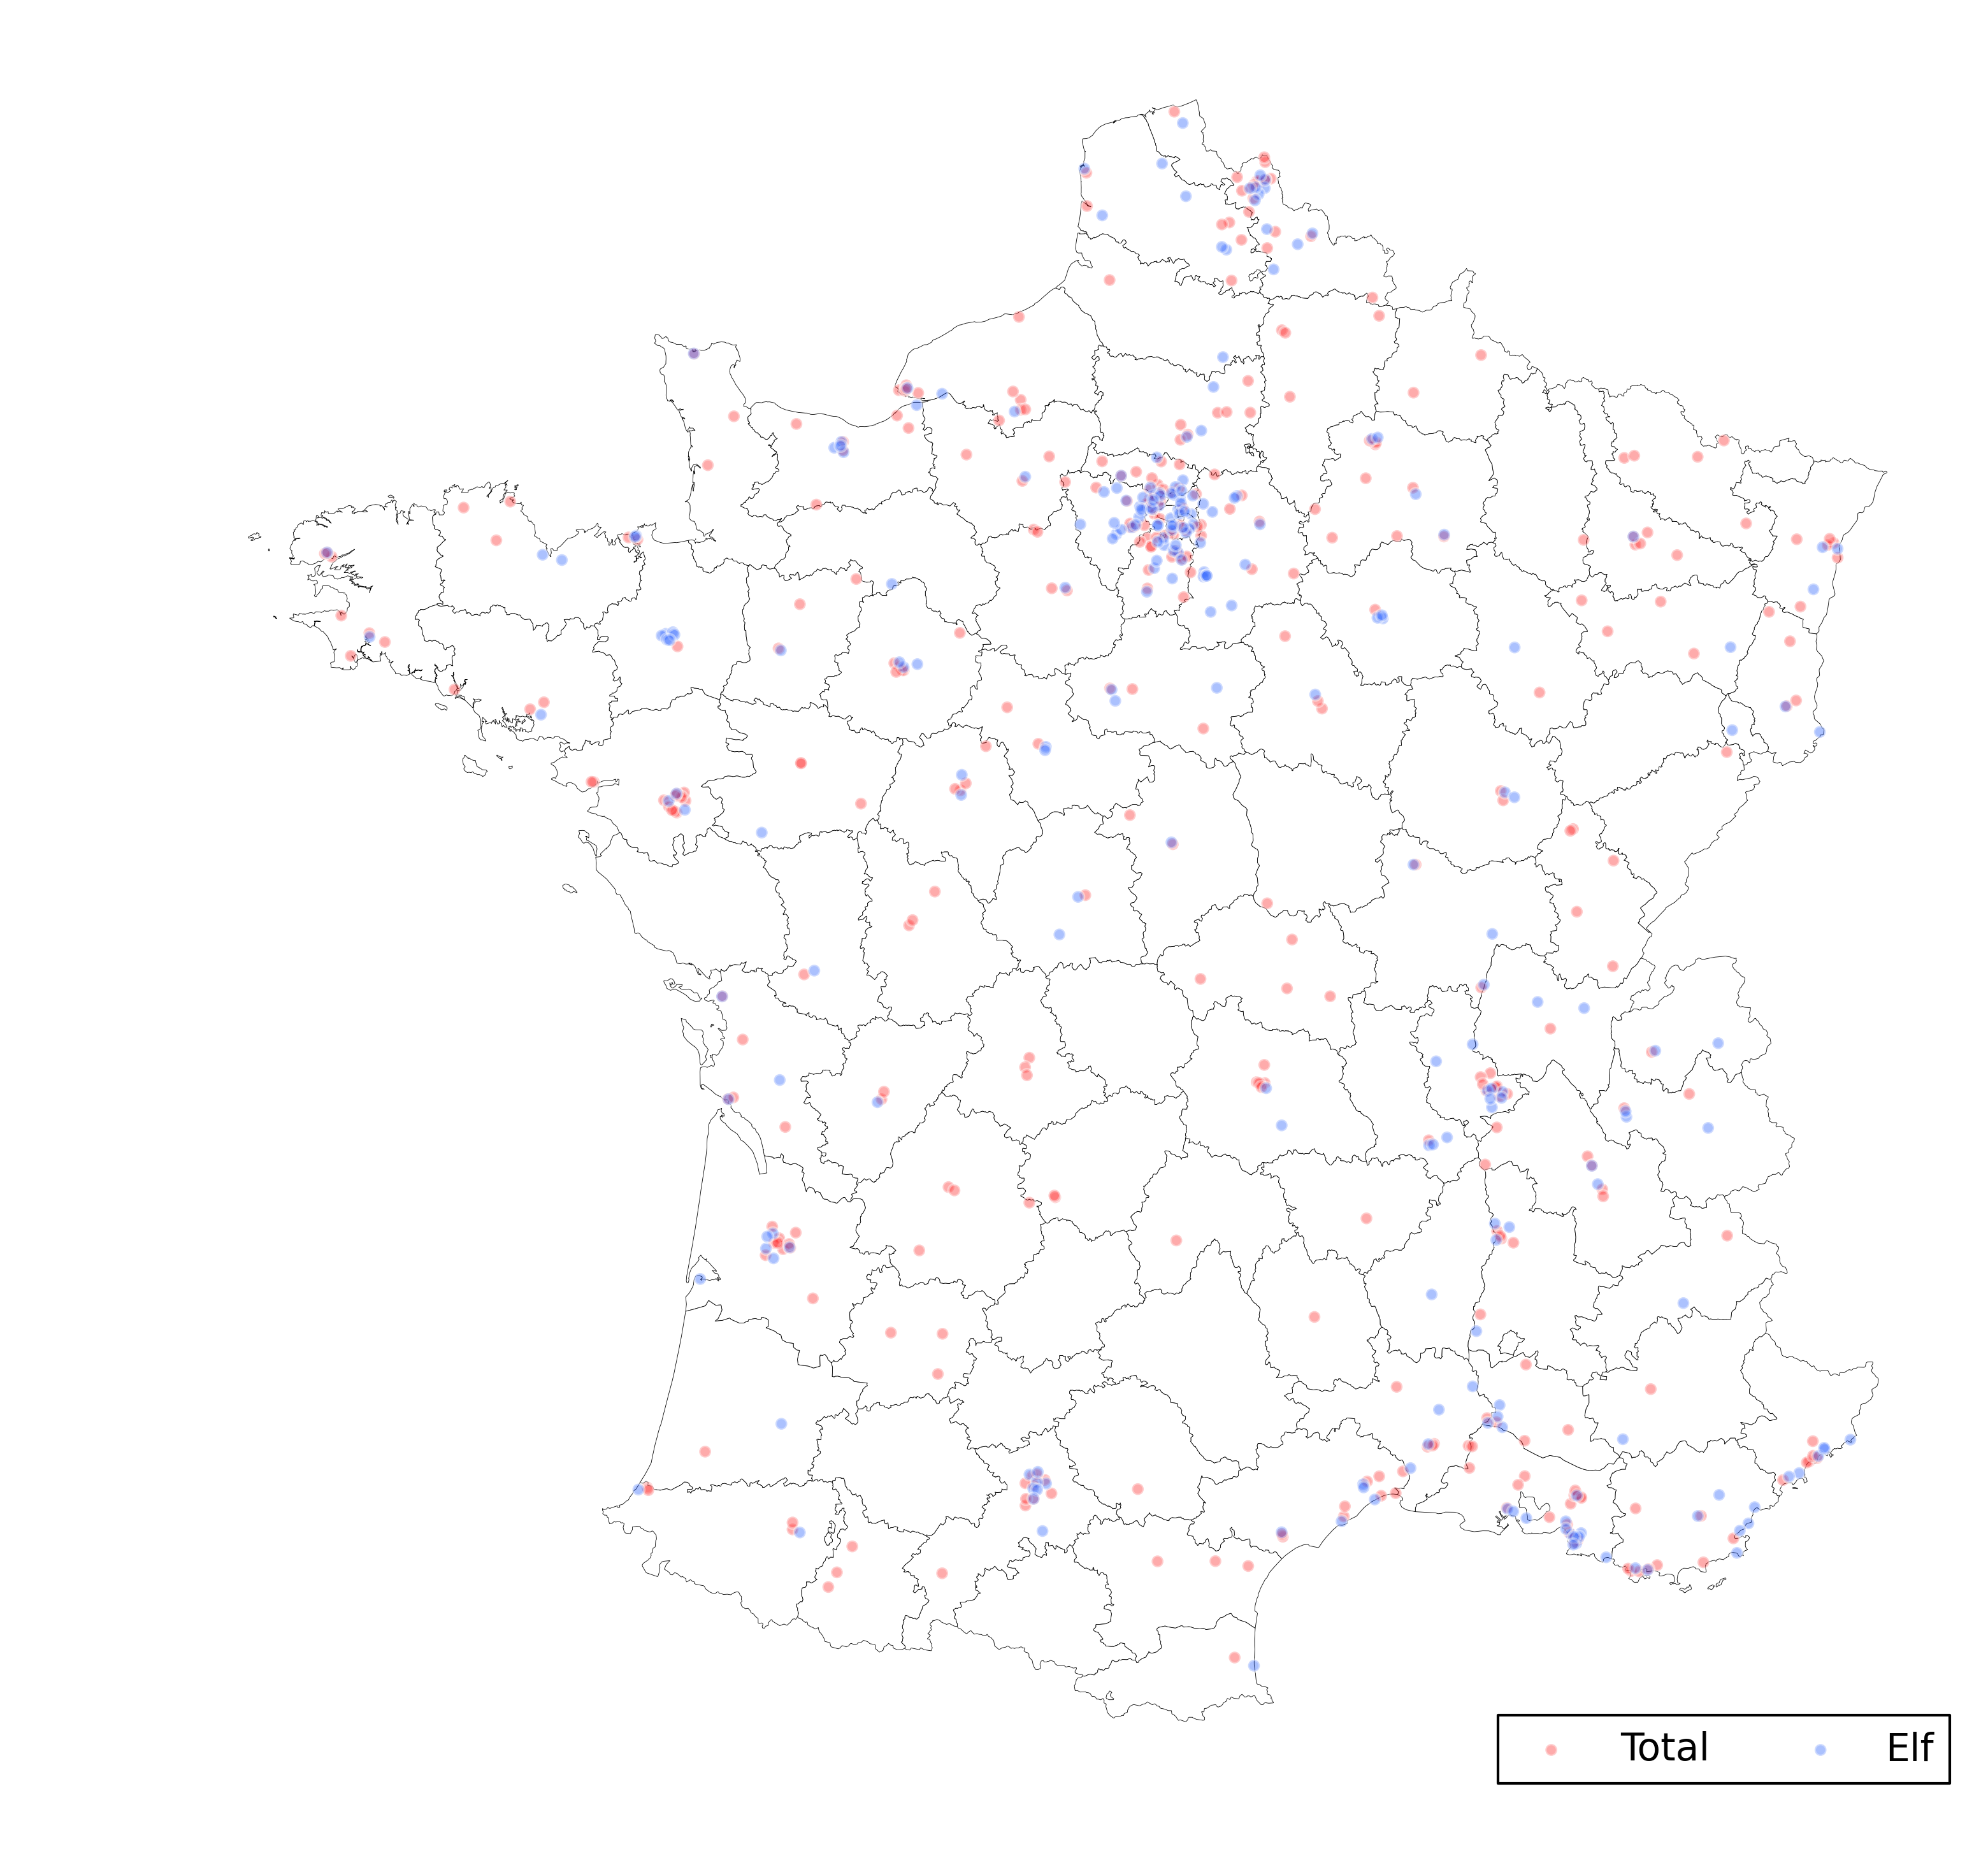
\includegraphics[width=16cm]{graphs/map_total_access.png}
	\floatfoot{}
\caption{Total Access gas stations end 2014}
\label{figure:map_ta}
\end{figure}


\end{document} 